\documentclass{beamer}

\mode<presentation> {
  \usetheme{PaloAlto}
}

%%
\makeatletter
\setbeamertemplate{subsubsection in sidebar}{\vspace*{-\baselineskip}}
\setbeamertemplate{subsubsection in sidebar shaded}{\vspace*{-\baselineskip}}
\makeatother
%%

%%
\setbeamertemplate{theorems}[numbered]
%%

\definecolor{Garnet}{RGB}{130,0,20}
\usecolortheme[named=Garnet]{structure}

\logo{
\includegraphics[width=1.5cm]{../../sharedImgs/USClogo.png}}

%\setbeamercolor{title}{fg=red!60!black,bg=white!50!black}
%\usecolortheme{beaver}
%\usecolortheme{crane}
\usefonttheme{structuresmallcapsserif}
\usefonttheme[onlysmall]{structurebold}

\usepackage{multicol}
\usepackage{graphicx}
\usepackage{mathtools}
\usepackage{latexsym}
\usepackage{amsfonts}
\usepackage[only,ninrm,elvrm,twlrm,sixrm,egtrm,tenrm]{rawfonts}
\usepackage{indentfirst}
\usepackage[noend]{algorithmic}
\usepackage{algorithm}
\usepackage{enumerate}
\usepackage{graphicx,psfrag}
\usepackage{epsfig}
%\usepackage[pdflatex]{graphicx}
%\usepackage{epstopdf}
\usepackage{ulem}
\usepackage{animate} %need the animate.sty file
\usepackage{tikz}
\usetikzlibrary{fit,shapes,calc}
\usepackage{pgfplots}
\usepackage{amsmath,amsthm,amssymb,amsfonts,enumerate,mymath,mathtools,tikz-cd,mathrsfs}

\newtheorem{thm}{Theorem}
\newtheorem{lem}{Lemma}
\newtheorem{prop}{Proposition}
\theoremstyle{definition}
\newtheorem{defn}{Definition}
\newtheorem{rmk}{Remark}

\newcommand{\A}{\mathscr{A}}
\renewcommand{\C}{\mathscr{C}}

\newcommand*{\defeq}{\mathrel{\vcenter{\baselineskip0.5ex \lineskiplimit0pt
                     \hbox{\scriptsize.}\hbox{\scriptsize.}}}%
                     =}
\DeclarePairedDelimiter\ceil{\lceil}{\rceil}
\DeclarePairedDelimiter\floor{\lfloor}{\rfloor}

\input epsf



\usepackage[english]{babel}
% or whatever

\usepackage[latin1]{inputenc}
% or whatever

\usepackage{times}
\usepackage[T1]{fontenc}
% Or whatever. Note that the encoding and the font should match. If T1
% does not look nice, try deleting the line with the fontenc.

\title % (optional, use only with long paper titles)
    {Functions}


\author[Farman]
{Blake Farman~\inst{1}}

\institute[USC]{
\inst{1}
University of South Carolina, Columbia, SC USA}
%\inst{2}
%East Carolina University, Greenville, NC USA\\
%\inst{3}
%University of Johannesburg, Auckland Park, South Africa}

\date[January 10, 2017]
{Math 122: Calculus for Business Administration and Social Sciences}

%\subject{Irredundant and Mixed Ramsey Numbers}
\setbeamercolor{alerted text}{fg=red!60!black}
\setbeamercolor{block title}{bg=white!50!black,fg=red!60!black}

\begin{document}

\begin{frame}
  \titlepage
\end{frame}

\begin{frame}
  \frametitle{Outline}
  \tableofcontents[pausesections]
\end{frame}

\section{1.1: Functions}

\begin{frame}{Definition}
  \begin{defn}
    \begin{itemize}
    \item<1->
      A {\it function} is a rule that takes certain values as inputs and assigns to each input {\bf exactly one} output.
    \item<2->
      The set of all possible inputs is called the {\it domain} of the function.
    \item<3->
      The set of all possible outputs is called the {\it range} of the function.
    \end{itemize}
  \end{defn}
  \pause
  \only<4->{Notation:
  A function named $f$ that takes as input the {\it independent variable}, $x$, and outputs the {\it dependent variable}, $y$, is written as
  $$y = f(x).$$}
\end{frame}

\begin{frame}{Example (Discrete Function)}
  \onslide<1->{Given any two sets we can define a function.}
  \onslide<2->{Say we have the sets
  $$D = \{1,2,3,4\}\ \text{and}\ R = \{5,6,7,8\}.$$}
  \onslide<3->{Define}
  \begin{multicols}{3}
      \begin{itemize}
      \item<3->
        f(1) = 6
      \item<4->
        f(2) = 5
      \item<5->
        f(3) = 8
      \item<6->
        f(4) = 7
      \end{itemize}
      \columnbreak
    \onslide<7->{
      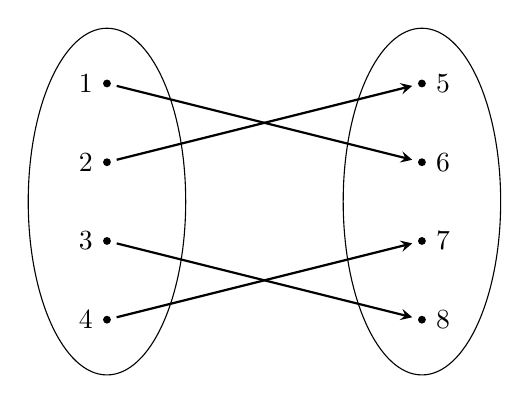
\begin{tikzpicture}[
     >=stealth,
     bullet/.style={
       fill=black,
       circle,
       minimum width=1pt,
       inner sep=1pt
     },
     projection/.style={
       ->,
       thick,
       shorten <=2pt,
       shorten >=2pt
     },
     every fit/.style={
       ellipse,
       draw,
       inner sep=0pt
     }
   ]
     \foreach \y/\l in {1/4,2/3/,3/2,4/1}
       \node[bullet,label=left:$\l$] (a\y) at (0,\y) {};
 
     \foreach \y/\l in {1/8,2/7,3/6,4/5}
       \node[bullet,label=right:$\l$] (b\y) at (4,\y) {};
 
     \node[draw,fit=(a1) (a2) (a3) (a4),minimum width=2cm] {} ;
     \node[draw,fit=(b1) (b2) (b3) (b4),minimum width=2cm] {} ;
 
     \onslide<7->{\draw[projection] (a1) -- (b2);}
     \onslide<8->{\draw[projection] (a2) -- (b1);}
     \onslide<9->{\draw[projection] (a3) -- (b4);}
     \onslide<10->{\draw[projection] (a4) -- (b3);}
   \end{tikzpicture}}
  \end{multicols}
\end{frame}

\begin{frame}{Example}
  The function $f(x) = x^2$ is a function.
  \begin{center}
    \begin{itemize}
    \item<2->
      The domain of $f$ is the set of all real numbers, $\R$.\\
    \item<3->
      The range of $f$ is the set of all non-negative real numbers,
      $$\left\{x \in \R \;\middle\vert\; 0 \leq x\right\}.$$
    \end{itemize}
  \end{center}
\end{frame}

\begin{frame}{Non-Example}
  The following depicts a non-function.
  \begin{center}
    \onslide<2->{
      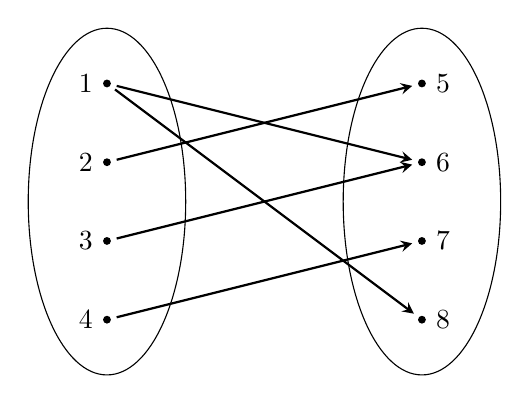
\begin{tikzpicture}[
          >=stealth,
          bullet/.style={
            fill=black,
            circle,
            minimum width=1pt,
            inner sep=1pt
          },
          projection/.style={
            ->,
            thick,
            shorten <=2pt,
            shorten >=2pt
          },
          every fit/.style={
            ellipse,
            draw,
            inner sep=0pt
          }
        ]
        \foreach \y/\l in {1/4,2/3/,3/2,4/1}
        \node[bullet,label=left:$\l$] (a\y) at (0,\y) {};
        
        \foreach \y/\l in {1/8,2/7,3/6,4/5}
        \node[bullet,label=right:$\l$] (b\y) at (4,\y) {};
        
        \node[draw,fit=(a1) (a2) (a3) (a4),minimum width=2cm] {} ;
        \node[draw,fit=(b1) (b2) (b3) (b4),minimum width=2cm] {} ;
        
        \onslide<7->{\draw[projection] (a4) -- (b1);}
        \onslide<6->{\draw[projection] (a1) -- (b2);}
        \onslide<5->{\draw[projection] (a2) -- (b3);}
        \onslide<4->{\draw[projection] (a3) -- (b4);}
        \onslide<3->{\draw[projection] (a4) -- (b3);}
    \end{tikzpicture}}
  \end{center}
  \onslide<8->{The value $f(1)$ is not well-defined because it requires a choice: it could be either 6 or 8.}
\end{frame}

\subsection{Graphs}

\begin{frame}{Cartesian Plane}
  Recall that the {\it Cartesian plane} is the set of all pairs
  $$\R^2 = \left\{(x,y) \;\middle\vert\; x \in \R, y \in \R\right\}.$$
  \pause
  It can be depicted as 
  \begin{center}
    \begin{tikzpicture}
      \begin{axis}
        [
          width=3in,
          axis equal image,
          clip=false,
          axis lines=middle,
          xmin=-5,
          xmax=5,
          ymin=-5,
          ymax=5,
          restrict y to domain=-5:5,
          xtick={\empty},
          ytick={\empty},
          axis line style={latex-latex},
          xlabel=$x$,
          ylabel=$y$,
          xlabel style={at={(ticklabel* cs:1)},anchor=north west},
          ylabel style={at={(ticklabel* cs:1)},anchor=south west},
        ]
      \end{axis}
    \end{tikzpicture}
  \end{center}
\end{frame}

\begin{frame}{Graph of a Function}
  \begin{defn}
    The graph of a real-valued function, $f$, with domain $D \subseteq \R$ is the set of pairs
    $$\left\{(x, f(x)) \;\middle\vert\; x \in D\right\} \subseteq \R^2.$$
    It can be drawn on the Cartesian plane.
  \end{defn}
\end{frame}

\begin{frame}{Example}
  The function $f(x) = x$ has 
  \begin{itemize}
    \item<2->
      Domain all real numbers, $\R$,
    \item<3->
      Range all real numbers, $\R$,
    \item<4->
      Graph $\left\{(x,x) \;\middle\vert\; x \in \R\right\}$,
      \onslide<5->
      \begin{center}
        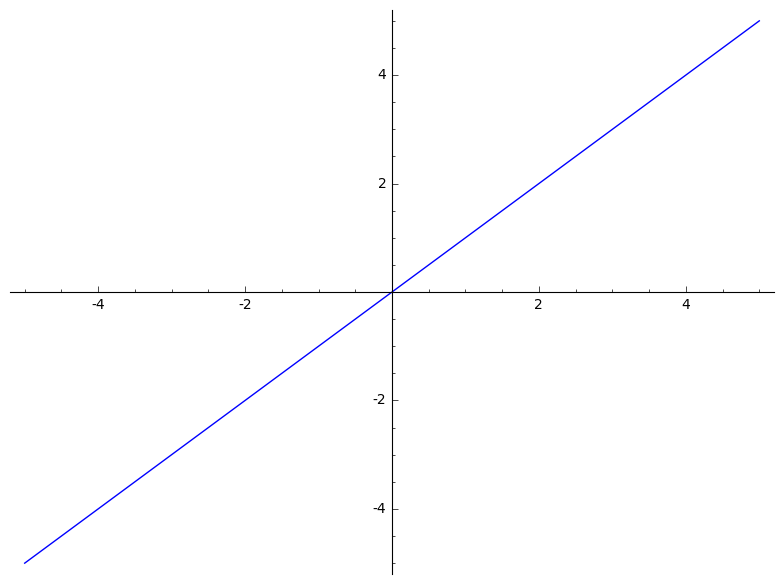
\includegraphics[scale=0.25]{imgs/idGraph.png}
      \end{center}
  \end{itemize}
\end{frame}


\begin{frame}{Increasing/Decreasing Functions}
  \begin{defn}
    Let $f$ be a function and let $[a,b]$ be an interval contained in the domain of $f$.
    We say $f$ is
    \begin{itemize}
      \item<2->
        {\it increasing on [a,b]} if $f(x_1) < f(x_2)$ whenever $a \leq x_1 < x_2 \leq b$,
      \item<3->
        {\it decreasing on [a,b]} if $f(x_2) < f(x_1)$ whenever $a \leq x_1 < x_2 \leq b$.
    \end{itemize}
    \onslide<4->
    We say that $f$ is increasing/decreasing if it is increasing/decreasing on its entire domain.
  \end{defn}
\end{frame}

\begin{frame}{Example}
  \begin{center}
    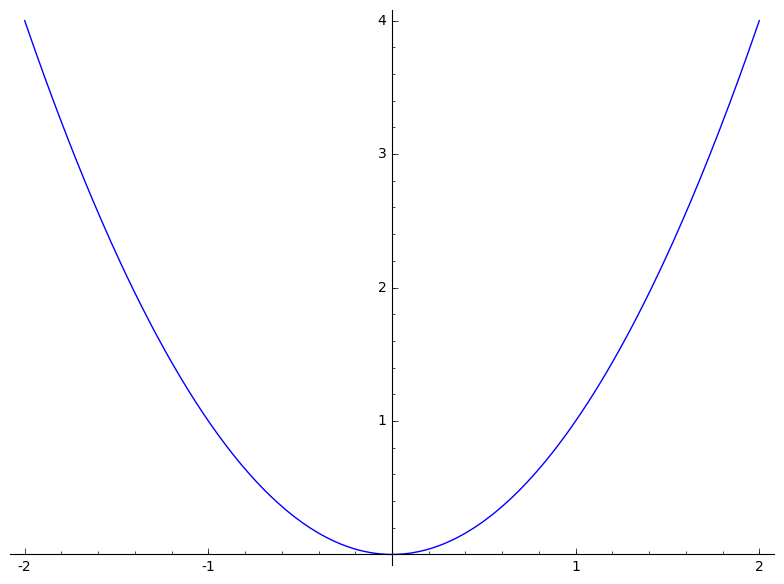
\includegraphics[scale=0.25]{imgs/parabola.png}
  \end{center}
  \begin{itemize}
  \item<2->
    Increasing on: \onslide<3->{$(0,\infty)$}
  \item<2->
    Decreasing on: \onslide<4->{$(-\infty,0)$}
  \end{itemize}
\end{frame}

\begin{frame}{Example}
  \begin{multicols}{2}
    
  \begin{center}
    Increasing\\
    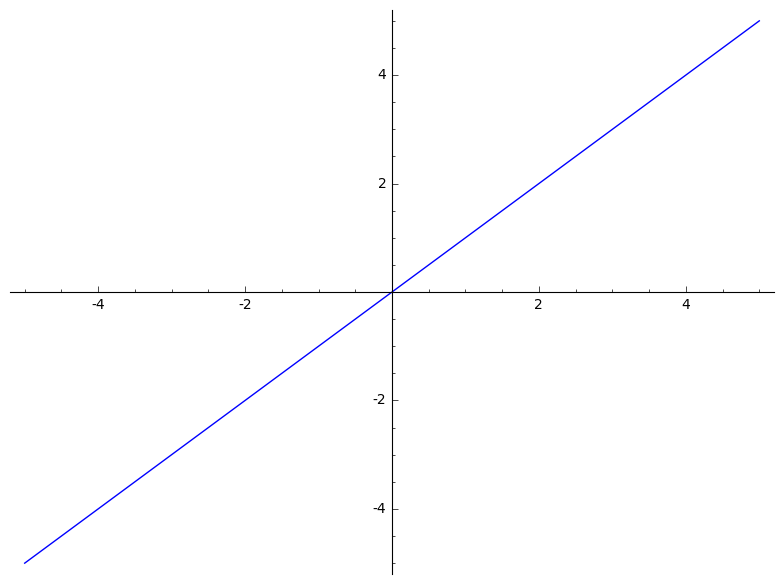
\includegraphics[scale=0.25]{imgs/idGraph.png}
  \end{center}
  \columnbreak
  \pause
  \begin{center}
    Decreasing\\
    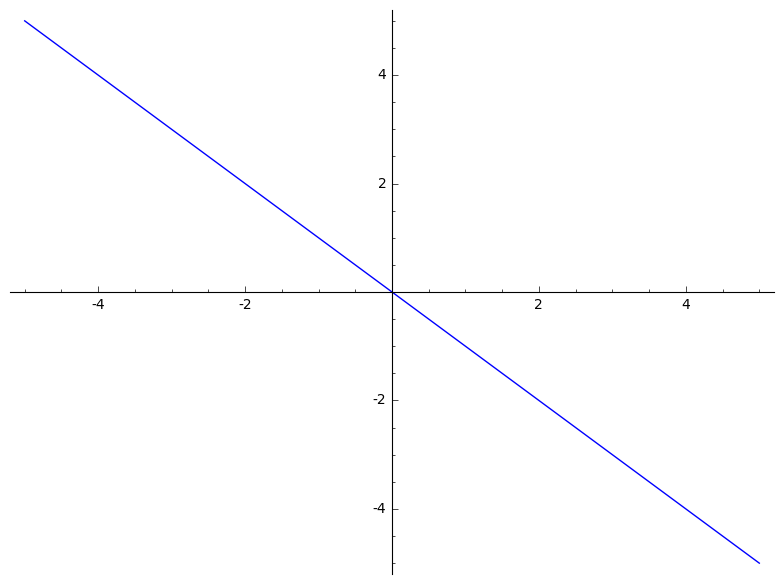
\includegraphics[scale=0.25]{imgs/negIdGraph.png}
  \end{center}
  \end{multicols}
\end{frame}

\begin{frame}{Intercepts}
  \begin{defn}
    Let $f$ be a function of a real variable, $x$.
    \begin{itemize}
      \item<2->
        The {\it $x$-intercepts} are the points $(x,0)$ on the graph.
      \item<3->
        The {\it $y$-intercept} is the point $(0,f(0))$ on the graph.
    \end{itemize}
  \end{defn}
\end{frame}

\begin{frame}{Example}
  Let $f(x) = x - 1$.\\
  \pause
  The $y$-intercept is
  $$(0,f(0)) = (0, 0 - 1) = (0,-1).$$\\
  \pause
  The $x-intercept$ is $(1,0)$:
  $$f(1) = 1 - 1 = 0.$$\\
  \pause
  \begin{center}
    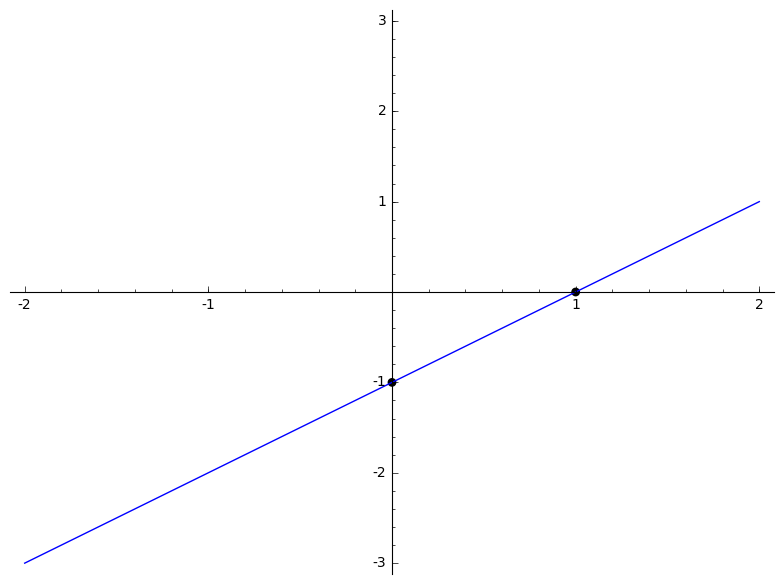
\includegraphics[scale=0.25]{imgs/intercepts}
  \end{center}
\end{frame}

\section{1.2: Linear Functions}

\begin{frame}{Definition}
  \begin{defn}
    A function, $f$, is {\it linear} if there exist real numbers $m$ and $b$ such that
    $$f(x) = mx + b.$$
    \begin{itemize}
    \item<2->
      Linear functions have domain and range $\R$,
    \item<3->
      The number $m$ is called the {\it slope} of the $f$,
    \item<4->
      The number $b$ is the $y$-intercept,
    \item<5->
      This form is usually called the {\it Slope-Intercept Form} of a line.
    \end{itemize}
  \end{defn}
\end{frame}

\begin{frame}{Graph of a Linear Function}
  The graph of $f(x) = mx + b$ is always a line.
  \pause
  They come in three flavors:
  \begin{itemize}
    \item<3->
      Increasing ($0 < m$):
      \begin{center}
        \begin{tikzpicture}
          \draw (0,0) -- (1,1);
        \end{tikzpicture}
      \end{center}
    \item<4->
      Decreasing ($m < 0$):
      \begin{center}
        \begin{tikzpicture}
          \draw (0,0) -- (1,-1);
        \end{tikzpicture}
      \end{center}
    \item<5->
      Horizontal ($m = 0$):
      \begin{center}
        \begin{tikzpicture}
          \draw (0,0) -- (1,0);
        \end{tikzpicture}
      \end{center}
  \end{itemize}
  
\end{frame}

\begin{frame}{Point-Slope Form}
  \begin{defn}
    Given: 
    \begin{itemize}
    \item<2->
      a point, $(x_0, y_0)$,
    \item<3->
      a slope, $m$,
    \end{itemize}
    \onslide<4->{
      the equation of the line through $(x_0,y_0)$ with slope $m$ is
      $$y - y_0 = m(x - x_0).$$
    }
  \end{defn}
\end{frame}

\begin{frame}{Two Points Determine a Line}
  Given two points, $(x_0, y_0)$ and $(x_1, y_1)$, the slope of the line passing through them is
  $$m = \frac{y_0 - y_1}{x_0 - x_1} = \frac{y_1 - y_0}{x_1 - x_0}.$$\\
  \pause
  The line passing through these two points is
  $$ y - y_0 = m(x - x_0)\ \text{or}\ y - y_1 = m(x - x_1).$$
  \pause
  To see these are the same line, put them both into Slope-Intercept Form.
\end{frame}

\begin{frame}{Two Points Determine a Line (Cont.)}
  \begin{eqnarray*}
    \onslide<1->{y &=& mx - \frac{y_0 - y_1}{x_0 - x_1}x_0 + y_0\\}
    \onslide<2->{&=& mx + \frac{(y_1 - y_0)x_0 + (x_0 - x_1)y_0}{x_0 - x_1}\\}
    \onslide<3->{&=& mx - \frac{x_0y_1 - x_1y_0}{x_0 - x_1}}
  \end{eqnarray*}
  \begin{eqnarray*}
    \onslide<1->{y &=& mx - \frac{y_0 - y_1}{x_0 - x_1} x_1 + y_1\\}
    \onslide<2->{&=& mx + \frac{(y_1 - y_0)x_1 + (x_0 - x_1)y_1}{x_0 - x_1}\\}
    \onslide<3->{&=& mx + \frac{x_0y_1 - x_1y_0}{x_0 - y_0}}
    \end{eqnarray*}
\end{frame}

\begin{frame}{Difference Quotients}
  \begin{defn}
    Let $f$ be a function.
    \onslide<2->{
    Given $x_0$, $x_1$ in the domain of $f$}\onslide<3->{, the {\it difference quotient} is
    $$\frac{f(x_1) - f(x_0)}{x_1 - x_0} = \frac{f(x_0) - f(x_1)}{x_0 - x_1}$$
    }
    \onslide<4->{
      This is just the slope of the line through $(x_0, f(x_0))$ and $(x_1, f(x_1))$.}
    \onslide<5->{
      This line is usually called the {\it Secant Line}}.
  \end{defn}
\end{frame}

\begin{frame}{Difference Quotients for Linear Functions}
  Let $f(x) = mx + b$.
  \onslide<2->{
  Given $x_0$ and $x_1$:
  }
  \begin{eqnarray*}
    \onslide<3->{\frac{f(x_1) - f(x_0)}{x_1 - x_0} &=& \frac{mx_1 + b - (mx_0 + b)}{x_1 - x_0}\\}
    \onslide<4->{&=& \frac{mx_1 - mx_0 + b - b}{x_1 - x_0}\\}
    \onslide<5->{&=& \frac{m(x_1 - x_0)}{x_1 - x_0}\\}
    \onslide<6->{&=& m}
  \end{eqnarray*}
  \onslide<7->{Hence for a linear function, the difference quotient is just the slope.}
\end{frame}

\begin{frame}{Difference Quotients for Non-Linear Functions}
  Let $f(x) = x^2$. For $x_0 = -1$, $x_1 = 2$:
  $$\onslide<2->{\frac{f(-1) - f(2)}{-1 - 2}} \onslide<3->{= \frac{(-1)^2 - 2^2}{-3}} \onslide<4->{= \frac{1 - 4}{-3}} \onslide<5->{= \frac{-3}{-3} = 1.}$$
  \onslide<6->{This is the slope of the secant line:}
  \begin{center}
      \onslide<6->{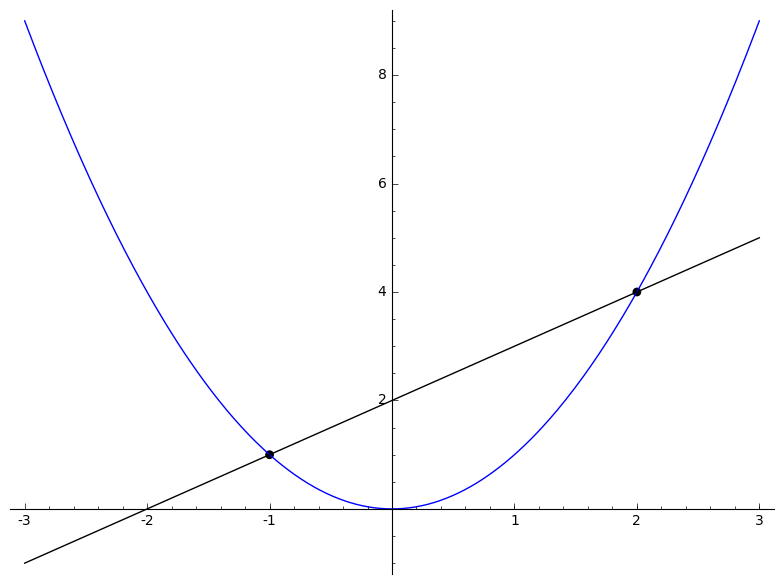
\includegraphics[scale=0.25]{imgs/diffQuo1.png}}
    \end{center}
\end{frame}

\begin{frame}{Difference Quotients for Non-Linear Functions (Cont.)}
  \onslide<1->{For $x_0 = 0$, $x_1 = 2$:}
  $$\onslide<2->{\frac{f(0) - f(2)}{0 - 2}} \onslide<3->{= \frac{0 - 4}{-2}} \onslide<4->{= \frac{4}{2} = 2.}$$
  \onslide<5->{This is the slope of the secant line:}
  \begin{center}
    \onslide<5->{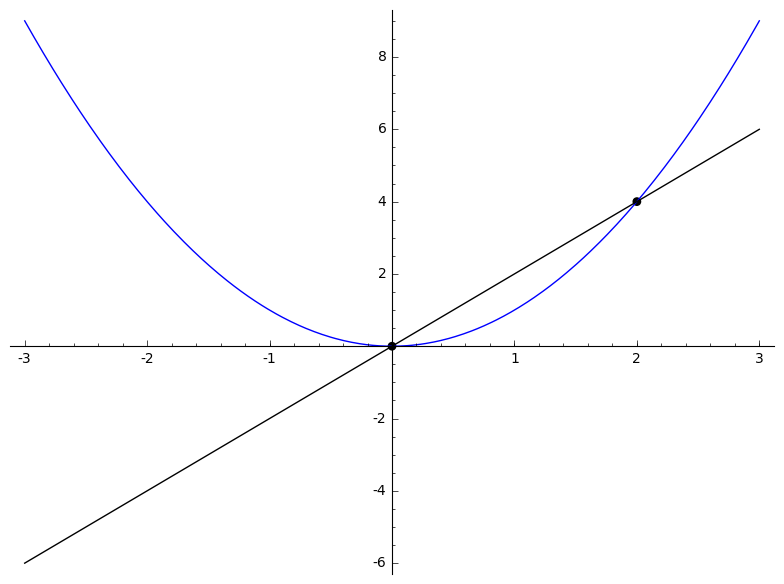
\includegraphics[scale=0.25]{imgs/diffQuo2.png}}
  \end{center}
\end{frame}

\end{document}
